%! TEX root = ../main.tex
\documentclass[../main.tex]{subfiles}

\begin{document}

\section{Risultati}

%... Per i 4 grafici seguenti, è stata utilizzata la sensibilità "candela". (era 0-1?)

\begin{figure}[ht!]
    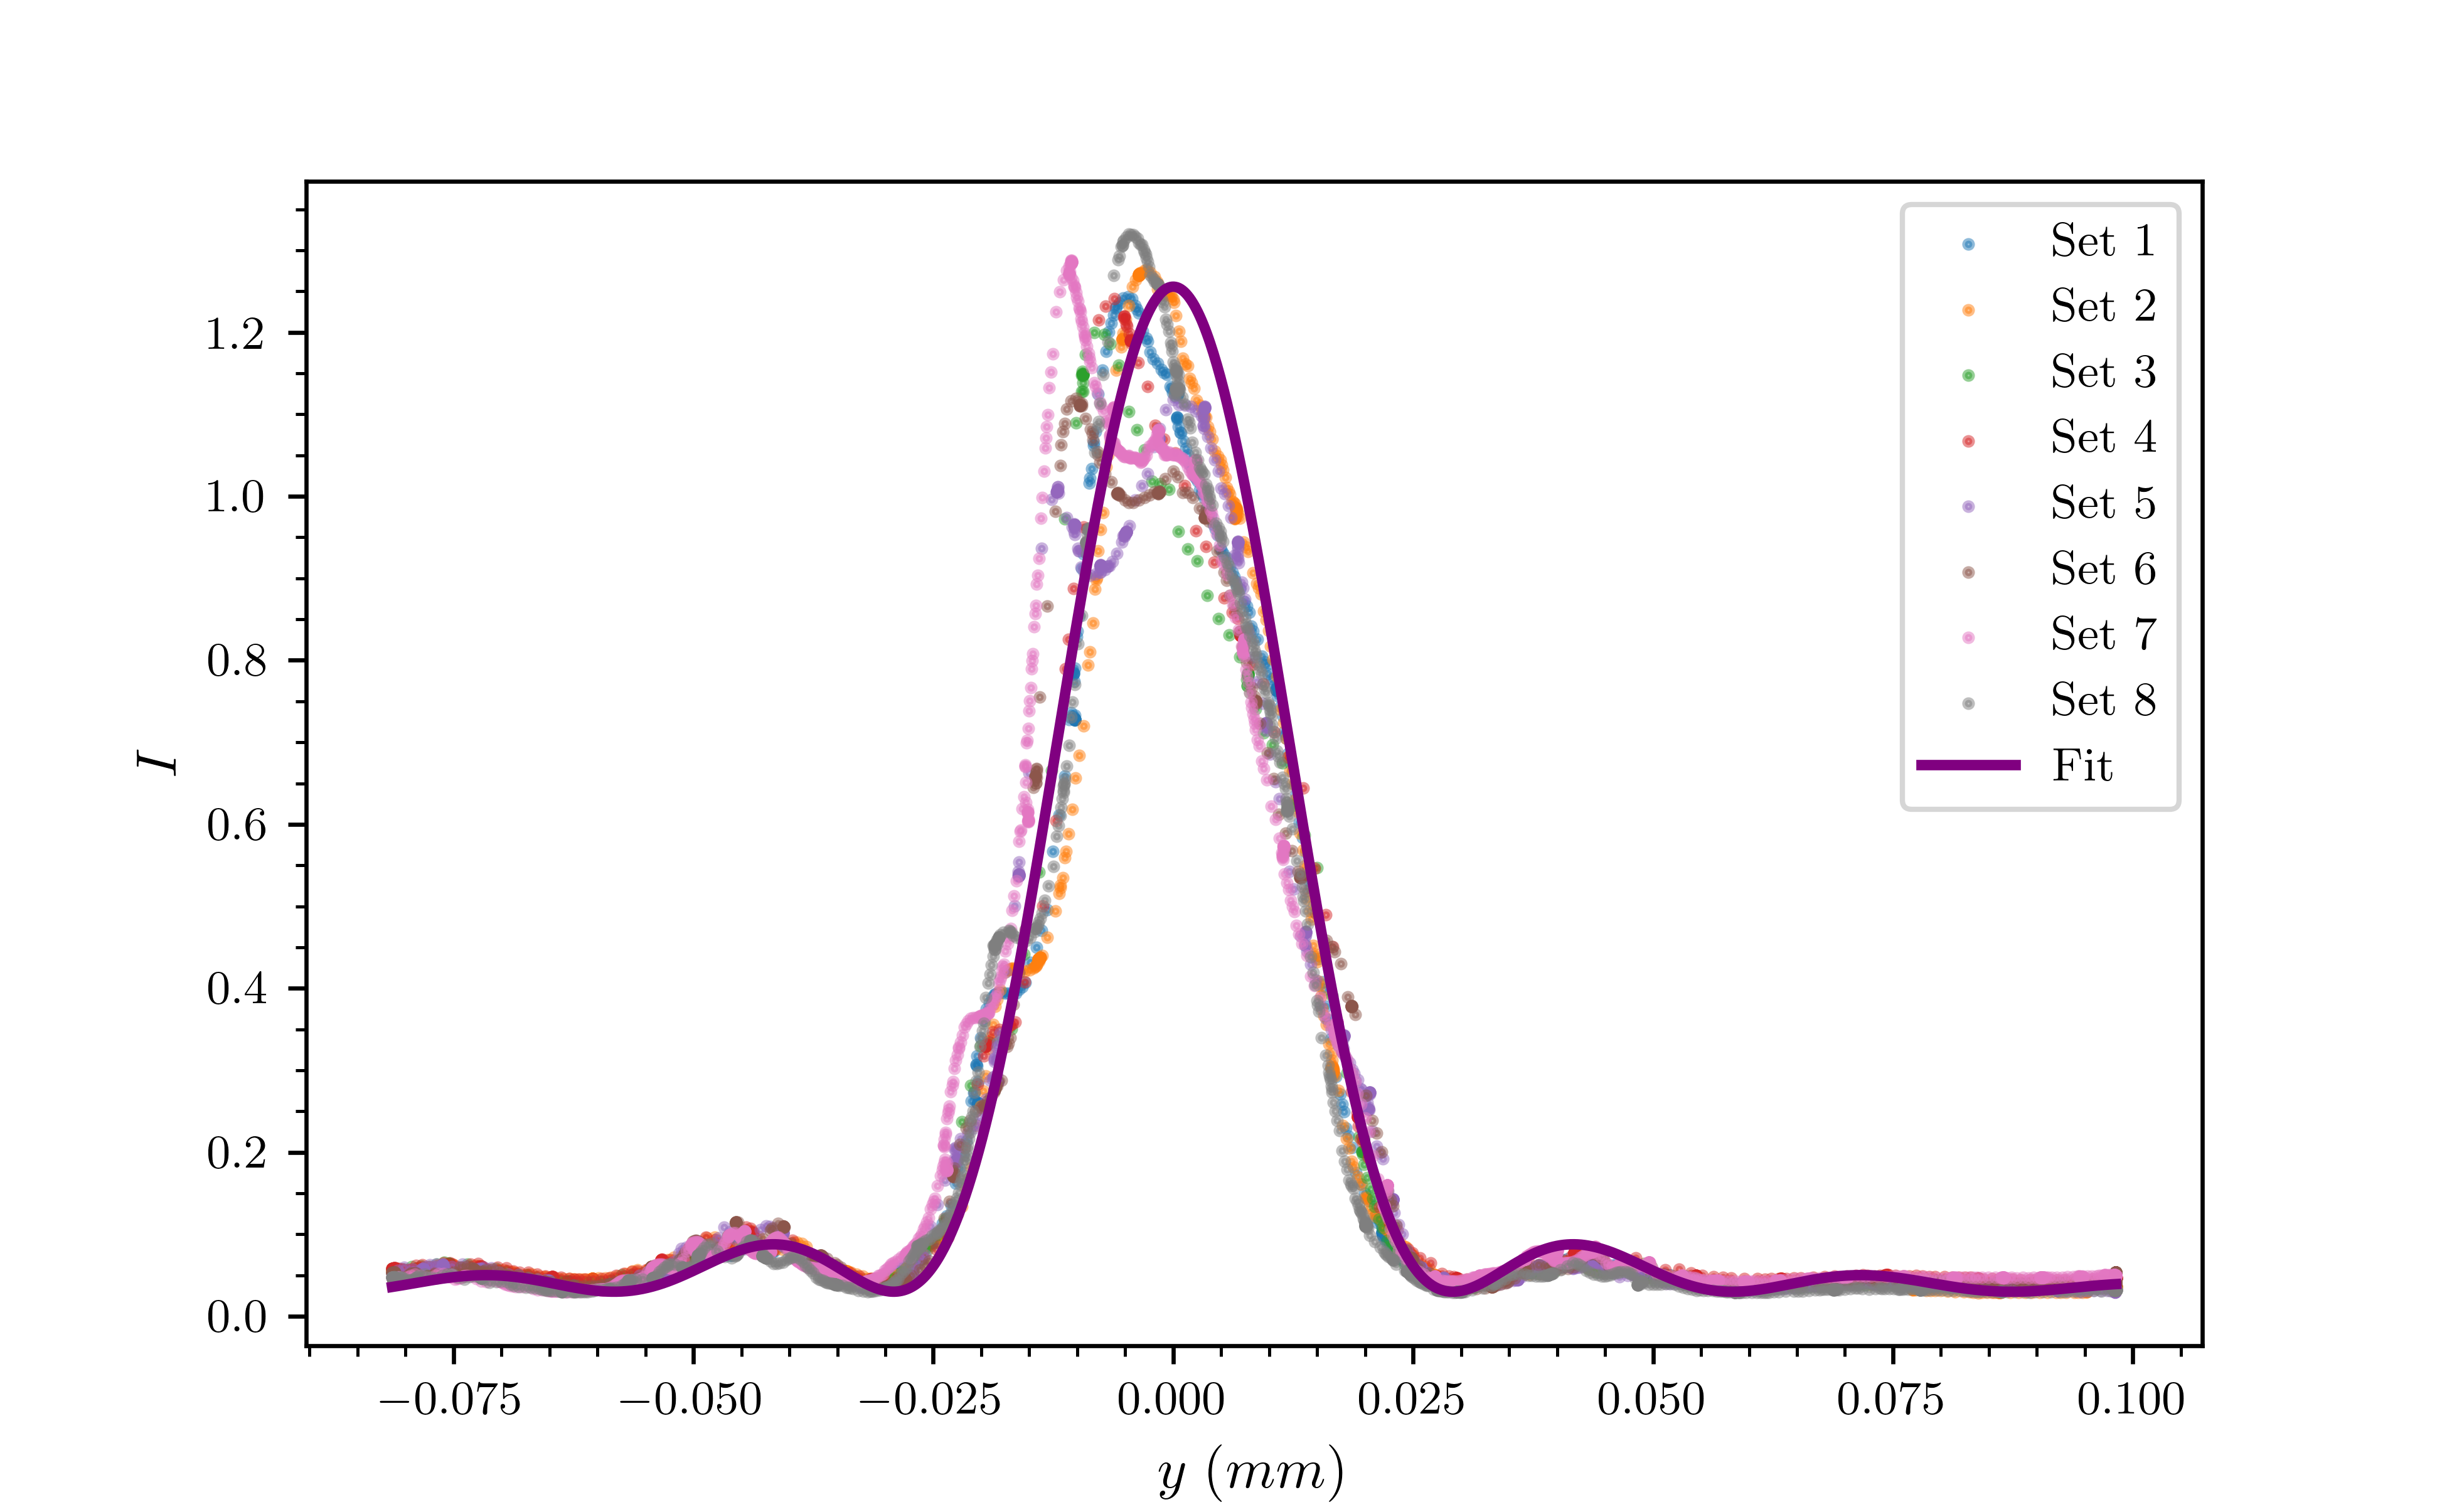
\includegraphics{../graphs/fit_0.02_1.5.png}
    \caption{Grafico dell’intensità della luce in funzione della posizione (cm). I set riportati sul grafico sono tre, ciascuno riferito ad un’apertura del detector di \num{1.5}, \num{1.0} e \qty{0.5}{\milli\meter}. In questo caso, la fenditura utilizzata è quella da \qty{0.02}{\milli\meter}. Si nota che i dati (in particolar modo quelli situati sul picco) non sono del tutto fedeli al fit.}
    \label{fig:fit_0.02_1.5}
\end{figure}

\begin{figure}[ht!]
    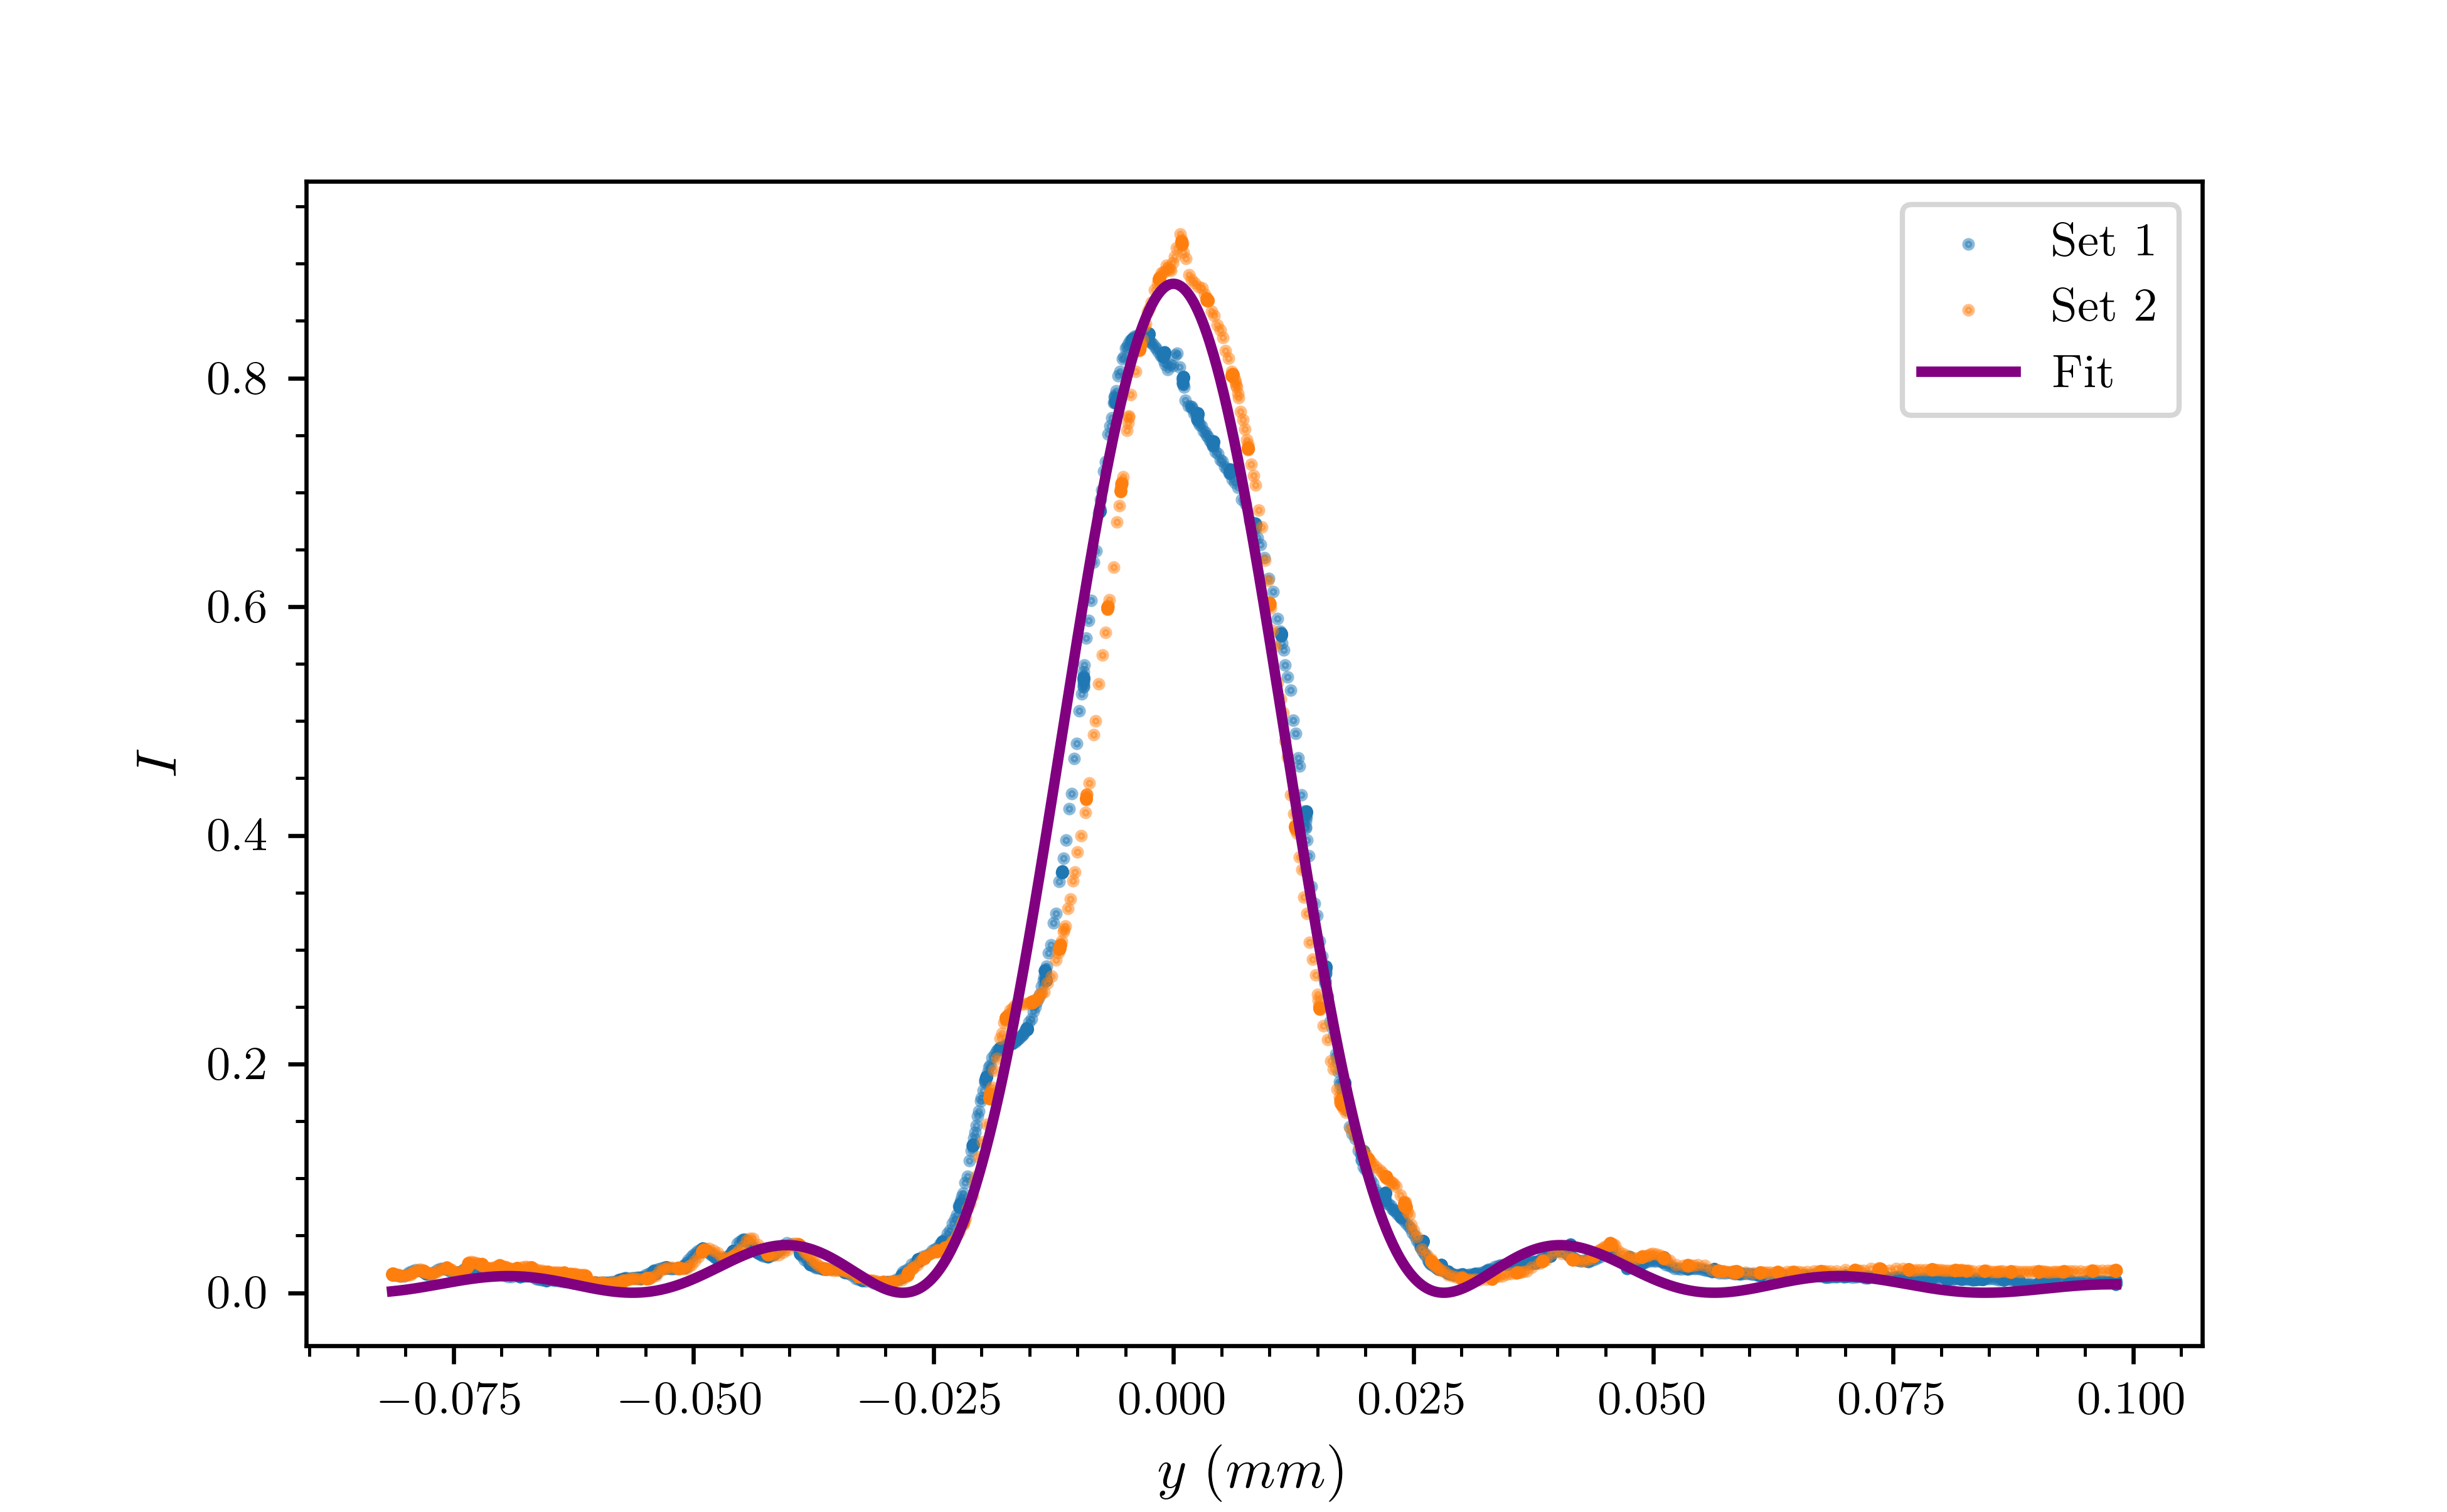
\includegraphics{../graphs/fit_0.02_1.0.png}
    \caption{}
    \label{fig:fit_0.02_1.0}
\end{figure}

\begin{figure}[ht!]
    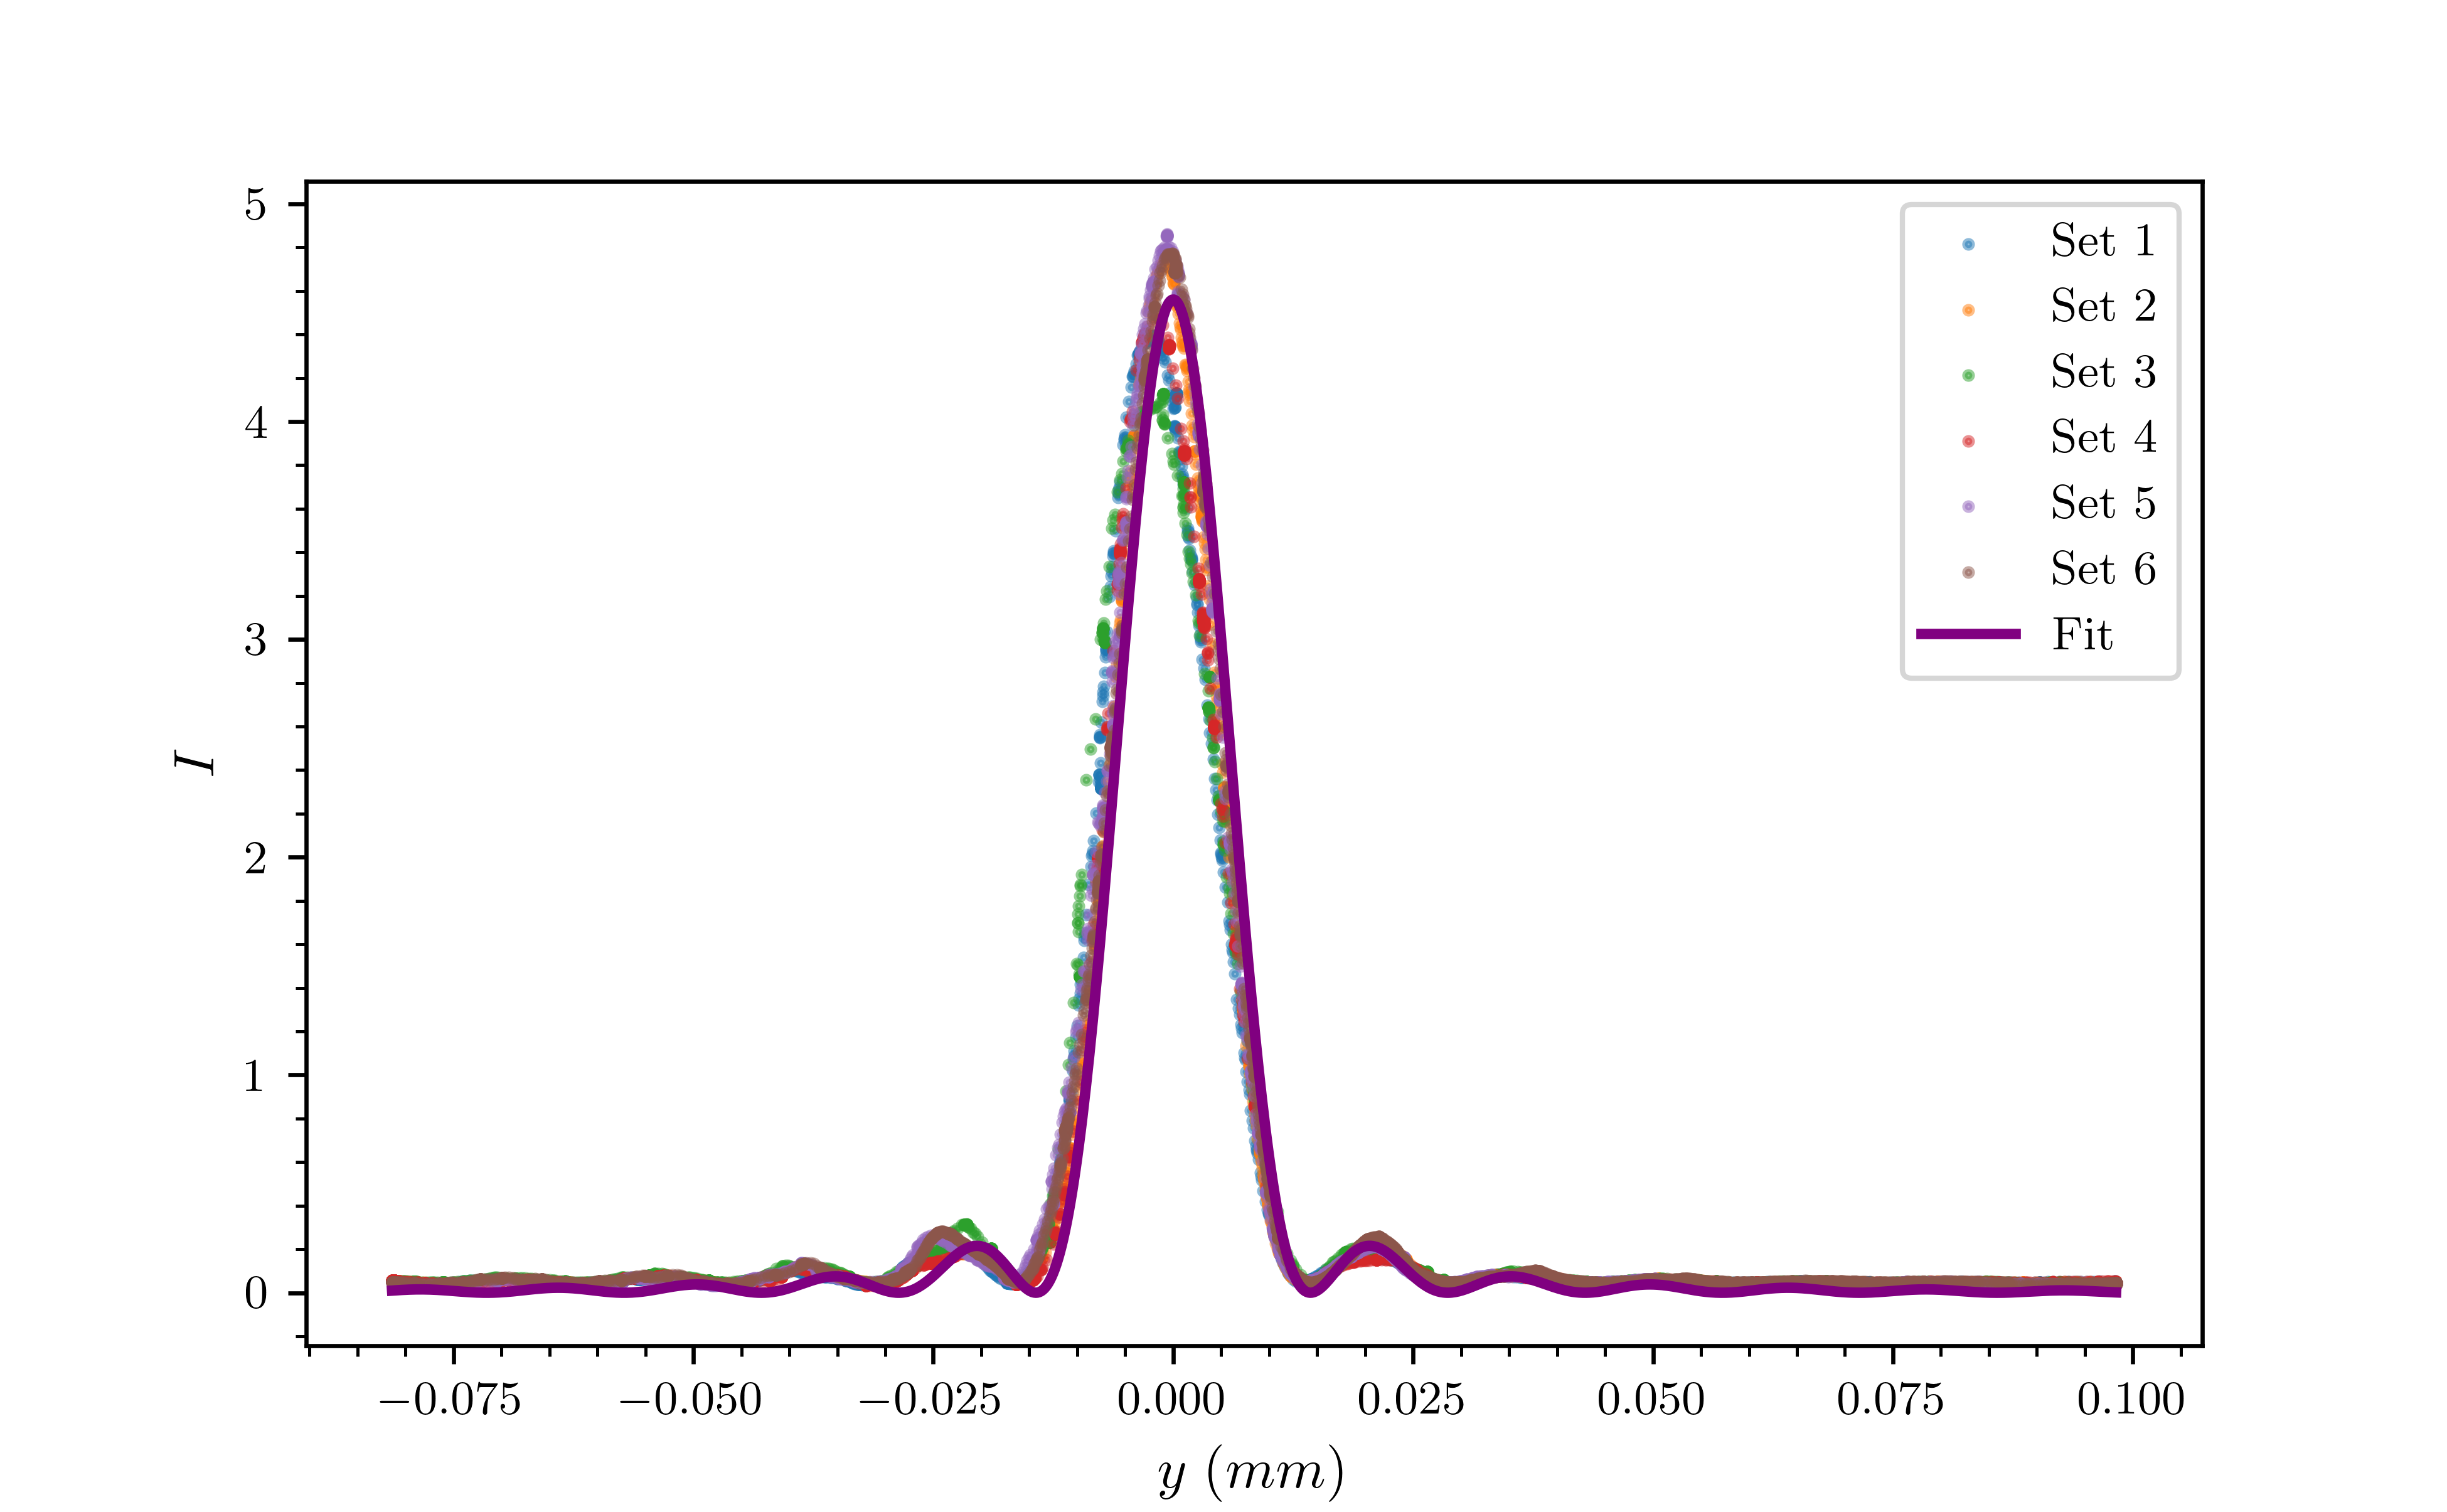
\includegraphics{../graphs/fit_0.04_1.5.png}
    \caption{Grafico dell’intensità della luce in funzione della posizione (cm). I set riportati sul grafico sono tre, ciascuno riferito ad un’apertura del detector di \num{1.5}, \num{1.0} e \qty{0.5}{\milli\meter}; in questo caso la fenditura utilizzata è quella da \qty{0.04}{\milli\meter}. Qui i dati presentano una migliore fedeltà alla forma del fit, nonostante ci sia un piccolo spostamento verso sinistra.}
    \label{fig:fit_0.04_1.5}
\end{figure}

\begin{figure}[ht!]
    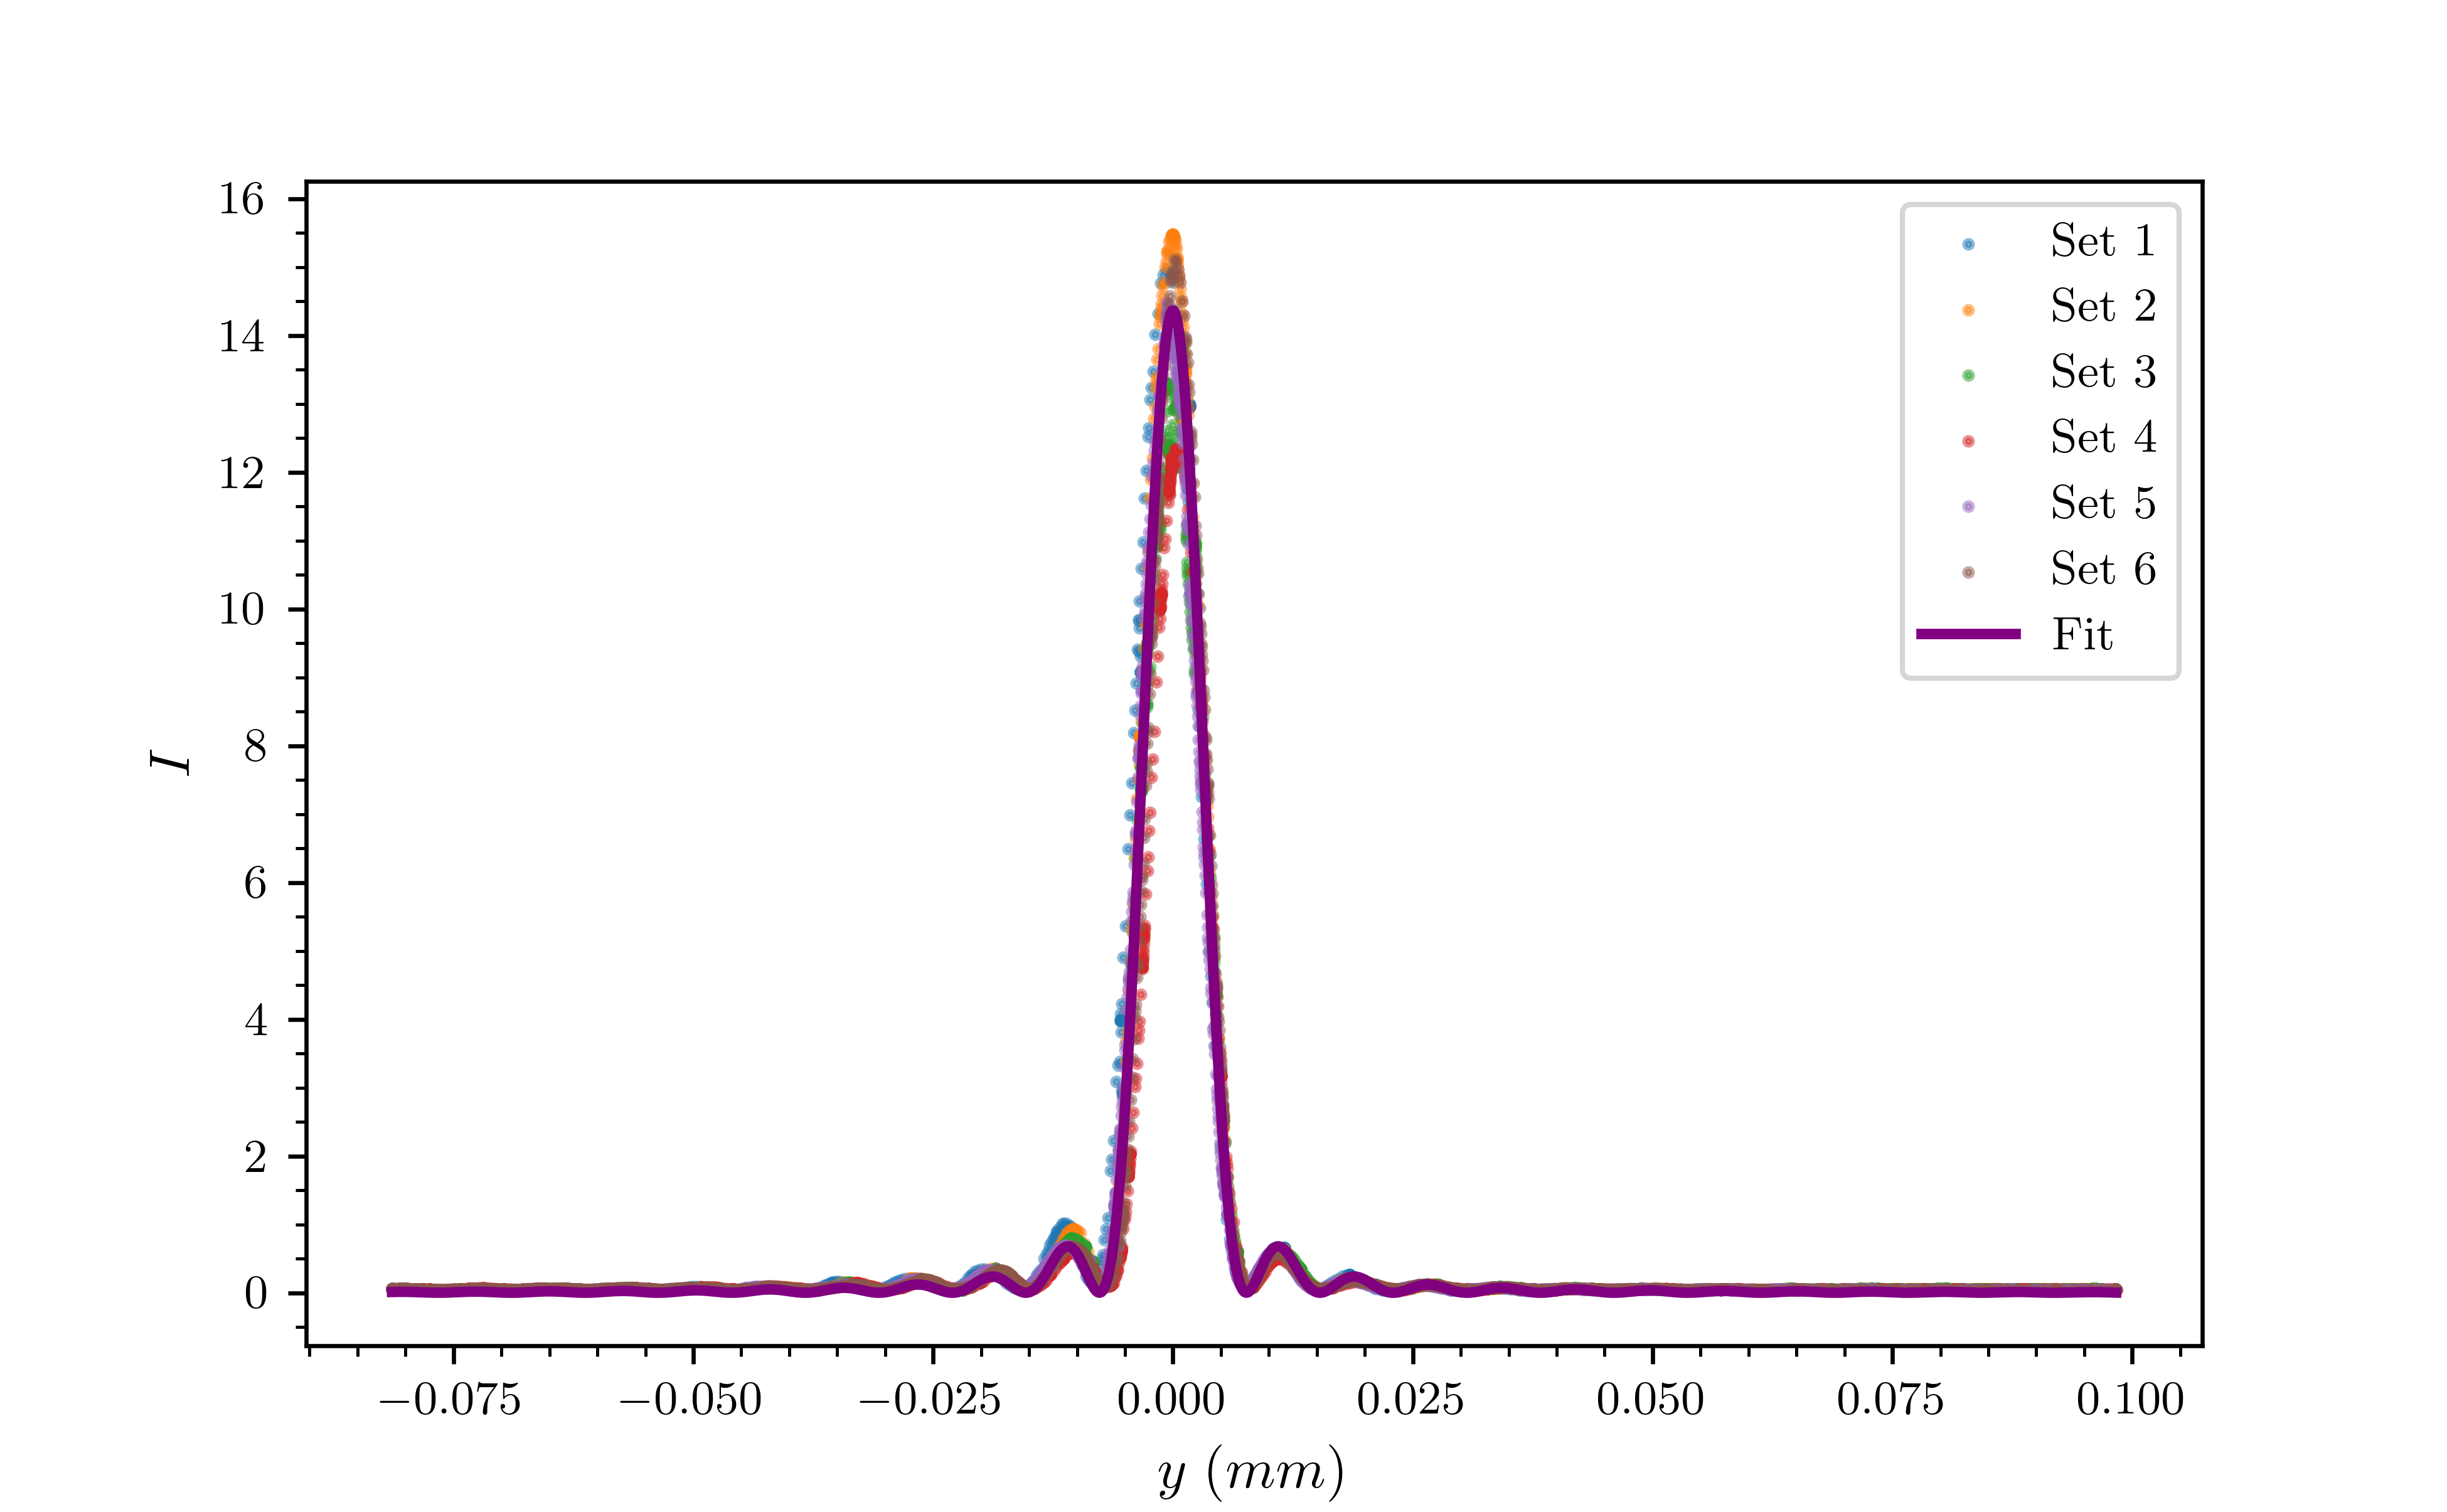
\includegraphics{../graphs/fit_0.08_1.5.png}
    \caption{Grafico dell’intensità della luce in funzione della posizione (cm). I set riportati sul grafico sono tre, ciascuno riferito ad un’apertura del detector di \num{1.5}, \num{1.0} e \qty{0.5}{\milli\meter}; in questo caso la fenditura utilizzata è quella da \qty{0.08}{\milli\meter}.}
    \label{fig:fit_0.08_1.5}
\end{figure}

%* Stavo per commentare i grafici sopra ma aspetto il "cambio di layout" eventualmente

Sul grafico seguente, ottenuto come media tra i vari set, si è proceduto a cercare i minimi. Per trovarne la posizione sulle ascisse, sono stati considerati degli intorni centrati sulla posizione teorica di ciascun minimo, data dall'\autoref{eq:y=0 values}, di raggio $\frac{\lambda L}{2 a}$. È bastato infine localizzare il punto di ordinata più bassa in ciascuno di questi intervalli, evidenziati nella (reference alla figura) da rette tratteggiate verticali.

% \begin{figure}[ht!]
%     \includegraphics{../graphs/}
%     \caption{Grafico utilizzato per l'acquisizione dei punti di minimo (punti di interferenza distruttiva).}
%     \label{fig:}
% \end{figure}

\end{document}